\definecolor{codegreen}{rgb}{0,0.6,0}
\definecolor{codegray}{rgb}{0.5,0.5,0.5}
\definecolor{codepurple}{rgb}{0.58,0,0.82}
\definecolor{backcolour}{rgb}{0.95,0.95,0.92}

\lstdefinestyle{mystyle}{
    backgroundcolor=\color{backcolour},   
    commentstyle=\color{codegreen},
    keywordstyle=\color{magenta},
    numberstyle=\tiny\color{codegray},
    stringstyle=\color{codepurple},
    basicstyle=\ttfamily\footnotesize,
    breakatwhitespace=false,         
    breaklines=true,                 
    captionpos=b,                    
    keepspaces=true,                 
    numbers=left,                    
    numbersep=5pt,                  
    showspaces=false,                
    showstringspaces=false,
    showtabs=false,                  
    tabsize=2
}

\lstset{style=mystyle}

\chapter{Assumptions} % Main chapter title
\section*{1.1 \hspace{1cm} The Problem}
Most countries have different methods to distribute electric power. In Italy, for example, a Power Plant produces electricity, which is sent to a High-Voltage Power Cabin via Power Lines travelling on Pylons. \\
The USA, however, has a different approach:
\begin{itemize}
    \item[1.] Electricity is made at a generating station by huge generators. Generating stations can use wind, coal, natural gas, or water.
    \item[2.] The current is sent through transformers to increase the voltage to push the power long distances.
    \item[3.] The electrical charge goes through high-voltage transmission lines that stretch across the country.
    \item[4.] It reaches a substation, where the voltage is lowered so it can be sent on smaller power lines.
    \item[5.] It travels through distribution lines to your neighborhood. Smaller transformers reduce the voltage again to make the power safe to use in our homes. These smaller transformers may be mounted on the poles, or sitting on the ground (they’re the big green boxes, called pad mount transformers).
    \item[6.] It connects to your house and passes through a meter that measures how much your family uses.
    \item[7.] The electricity goes to the service panel in your basement or garage, where breakers or fuses protect the wires inside your house from being overloaded. (Never touch a service panel!  It is only to be operated by your parents or a professional.)
    \item[8.] The electricity travels through wires inside the walls to the outlets and switches all over your house.
\end{itemize}
Because this difference, only entities common to every country will be stored:
\begin{itemize}
    \item Power Plants
    \item Pylons
    \item (High-Voltage) Electric Cabins
    \item Power Lines
\end{itemize}

The Software will allow the system administrators to perform CRUD operations (Create, Read, Update, Delete) operations on the entities.

\section*{1.2 \hspace{1cm} The Company}
The only thing we know about the company is that it is an electricity distribution company. Since the task describes it as "the company" and there is no known national constraint, I assume that the company has a monopoly on all the electricity market in the world, just to work on the worst-case-scenario. \\

I assume that the data to be added to the archive also includes the power plants and the power lines. \\

Since there is no constraint on how the location should be stored, I will use the GPS coordinates system. \\

Since it's not specified who can access the archive, I assume that only the system administrators should access it. The system administrators can insert and delete data directly from the archive's web page (https://admin.electrocorp.com/archive), which only allows them to access it. \\

The archive will be initialized with official data from sources like NASA, data.europa.eu, etc., and will be cited in the source code.

TODO: wasd

\section*{1.3 \hspace{1cm} The Infrastructure}
The Company has different workplaces around the world, the servers are underwater (\href{https://datacenterfrontier.com/microsoft-servers-in-our-underwater-data-center-are-super-reliable/#:~:text=Microsoft%3A%20Servers%20in%20Our%20Underwater%20Data%20Center%20Are%20Super%2DReliable,-By%20Rich%20Miller&text=Microsoft%20recently%20retrieved%20the%20Project,the%20Orkney%20Islands%20in%20Scotland}{like Microsoft does}) for efficiency and cost reasons, and are divided in different subdomains, all connected to the same database. \\
The DBMS used is PostgreSQL, because it's super-scalable, and allows us to have a database cluster. \\

There are different subdomains, but the ones developed in this project are:
\begin{itemize}
    \item https://www.electrocorp.com/
    \item https://admin.electrocorp.com/
    \item https://api.electrocorp.com/
    \item https://mail.electrocorp.com/
\end{itemize}
(www.electrocorp.com is already taken by a company, and is not affilated with this project. the domain name is overwritten in my /etc/hosts file to point to my project, please do not connect to it externally). \\ \\
The servers are running SUSE Linux, an Enterprise GNU/Linux distribution for Servers.

The network is composed of different subnetworks, one for each cluster managed by Kubernetes. \\
Each subnetwork has different firewall rules, listed here:
\begin{center}
    \begin{tabular}{ |l|c|c|c|c|c| } 
        \hline
        \multicolumn{6}{|c|}{Firewall on www.electrocorp.com} \\
        \hline
            Number & Protocol & Source IP     & Destination IP & Destination Port & Action \\
        \hline
            4      & ALL      & 0.0.0.0/0    & 0.0.0.0/0     & 0-65535          & ACCEPT \\
        \hline
    \end{tabular}
\end{center}
    
\begin{center}
    \begin{tabular}{ |l|c|c|c|c|c| } 
        \hline
        \multicolumn{6}{|c|}{Firewall on admin.electrocorp.com} \\
        \hline
            Number & Protocol & Source IP     & Destination IP & Destination Port & Action \\
        \hline
            1      & TCP      & 172.22.3.0/24 & 172.22.4.0/24  & 5432             & ACCEPT \\
            2      & TCP      & 32.1.0.0/16   & 172.22.3.0/24  & 443              & ACCEPT \\
            3      & ALL      & 0.0.0.0/0    & 0.0.0.0/0     & 0-65535          & DROP \\
        \hline
    \end{tabular}
\end{center}

\begin{center}
    \begin{tabular}{ |l|c|c|c|c|c| } 
        \hline
        \multicolumn{6}{|c|}{Firewall on api.electrocorp.com} \\
        \hline
            Number & Protocol & Source IP     & Destination IP & Destination Port & Action \\
        \hline
            4      & ALL      & 0.0.0.0/0    & 172.22.2.5     & 0-65535          & ACCEPT \\
        \hline
    \end{tabular}
\end{center}

The subnet 32.1.0.0/16 is owned by the company and is used to allow employees to acces the administrative page.

\begin{center}
    \begin{tabular}{ |l|c|c|c|c|c| } 
        \hline
        \multicolumn{6}{|c|}{Firewall on the DBMS cluster} \\
        \hline
            Number & Protocol & Source IP     & Destination IP & Destination Port & Action \\
        \hline
            1      & TCP      & 172.22.2.0/24 & 172.22.4.0/24  & 5432             & ACCEPT \\
            2      & TCP      & 172.22.4.0/24 & 172.22.4.0/24  & 5432             & ACCEPT \\
            3      & ALL      & 0.0.0.0/0    & 0.0.0.0/0     & 0-65535          & DROP  \\
        \hline
    \end{tabular}
\end{center}
And here is the firewall configuration on a GNU/Linux router.

\lstinputlisting{Code/networking.sh}

The hosts on the same subnetwork can only connect to each other on the DBMS cluster. \\

Here is the docker-compose.yml configuration file, that also specifies the networking configuration.

\lstinputlisting{../../../project/docker-compose.yml}

... and the /etc/hosts file (C: \textbackslash Windows \textbackslash system32 \textbackslash etc \textbackslash hosts)
\lstinputlisting{/etc/hosts}

\section*{1.4 \hspace{1cm} The Website}
The archive is accessible at https://admin.electrocorp.com/archive by the system administrators only, and the page allows them to browse, add, remove, and update data from the archive. \\

The System Administrators also have the power to manage roles and users. \\


Here are the Access Control rules for the users on each website.
\begin{center}
    \begin{tabular}{ |l|c|c|c|c|c| } 
        \hline
        \multicolumn{6}{|c|}{Access Control (admin.electrocorp.com)} \\
        \hline
                                        & Archive    & Control Panel            & Login        & Finances                & Logs \\
        \hline
            \textbf{Administrator}      & ALL        & ALL                      & AUTHENTICATE & ALL                     & READ \\
            \textbf{Finances}           &            &                          & AUTHENTICATE & ALL                     &  \\
            \textbf{*not auth*}         &            &                          & AUTHENTICATE &                         &  \\
        \hline
    \end{tabular}
\end{center}
This is only accessible by the employees. \\


This is the block diagrams. \\
% \begin{center}
%     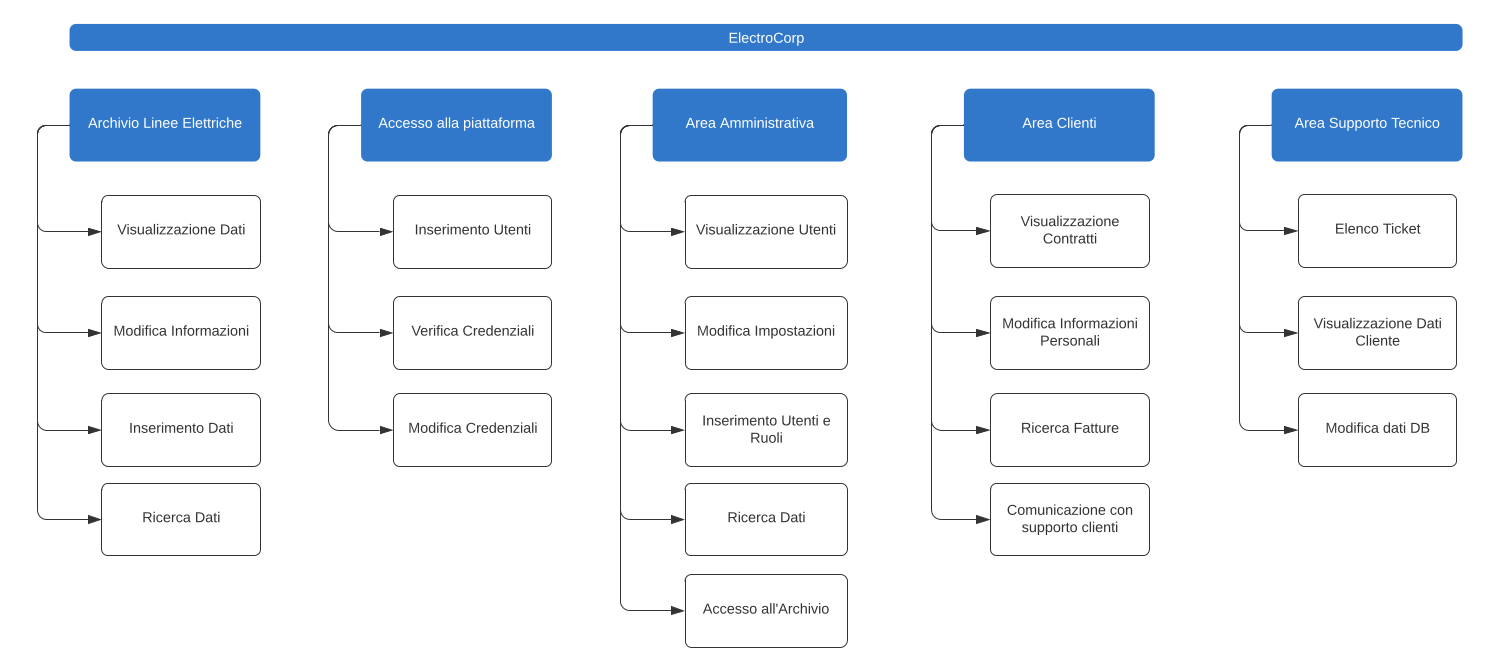
\includegraphics[width=\linewidth]{Figures/blocks.png}
% \end{center}
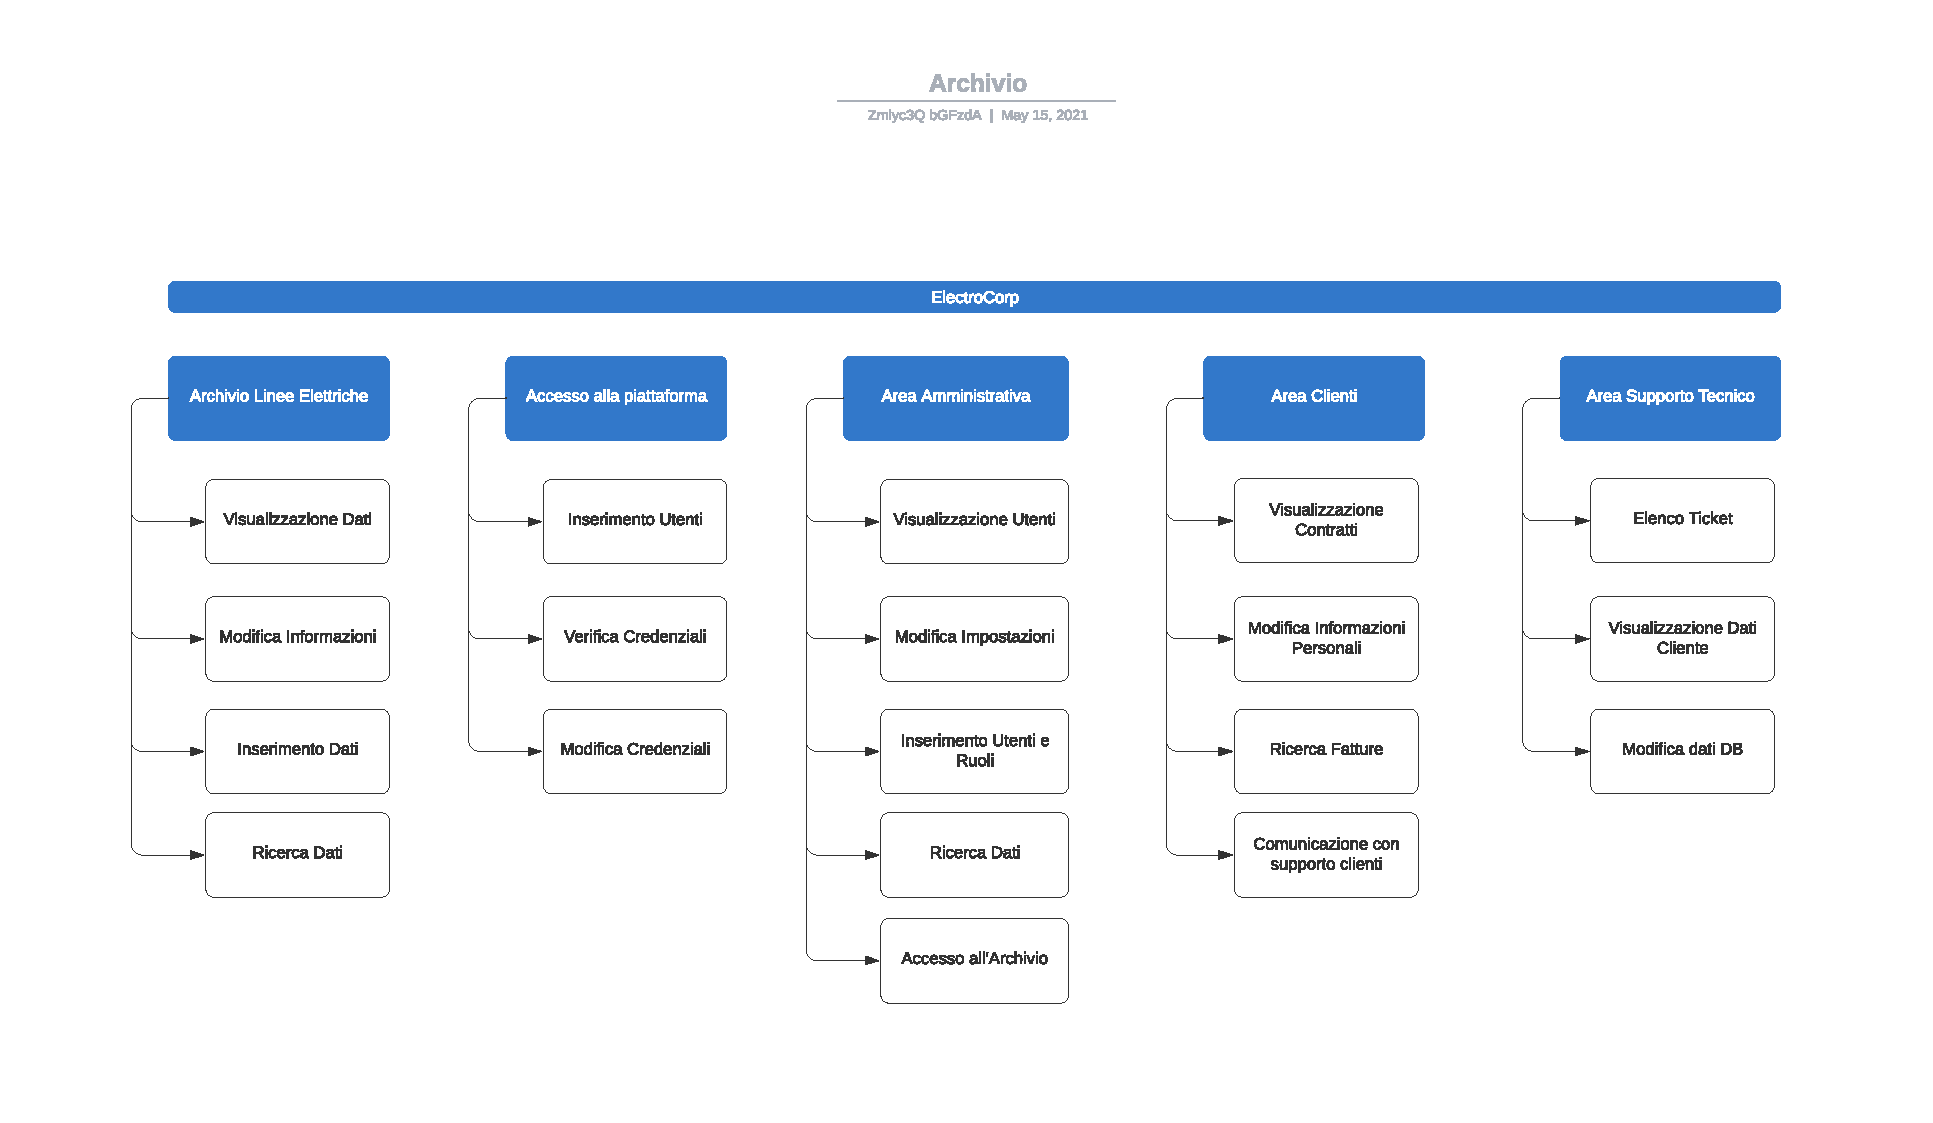
\includepdf{Figures/blocks.pdf}

And this is a Flow Chart.
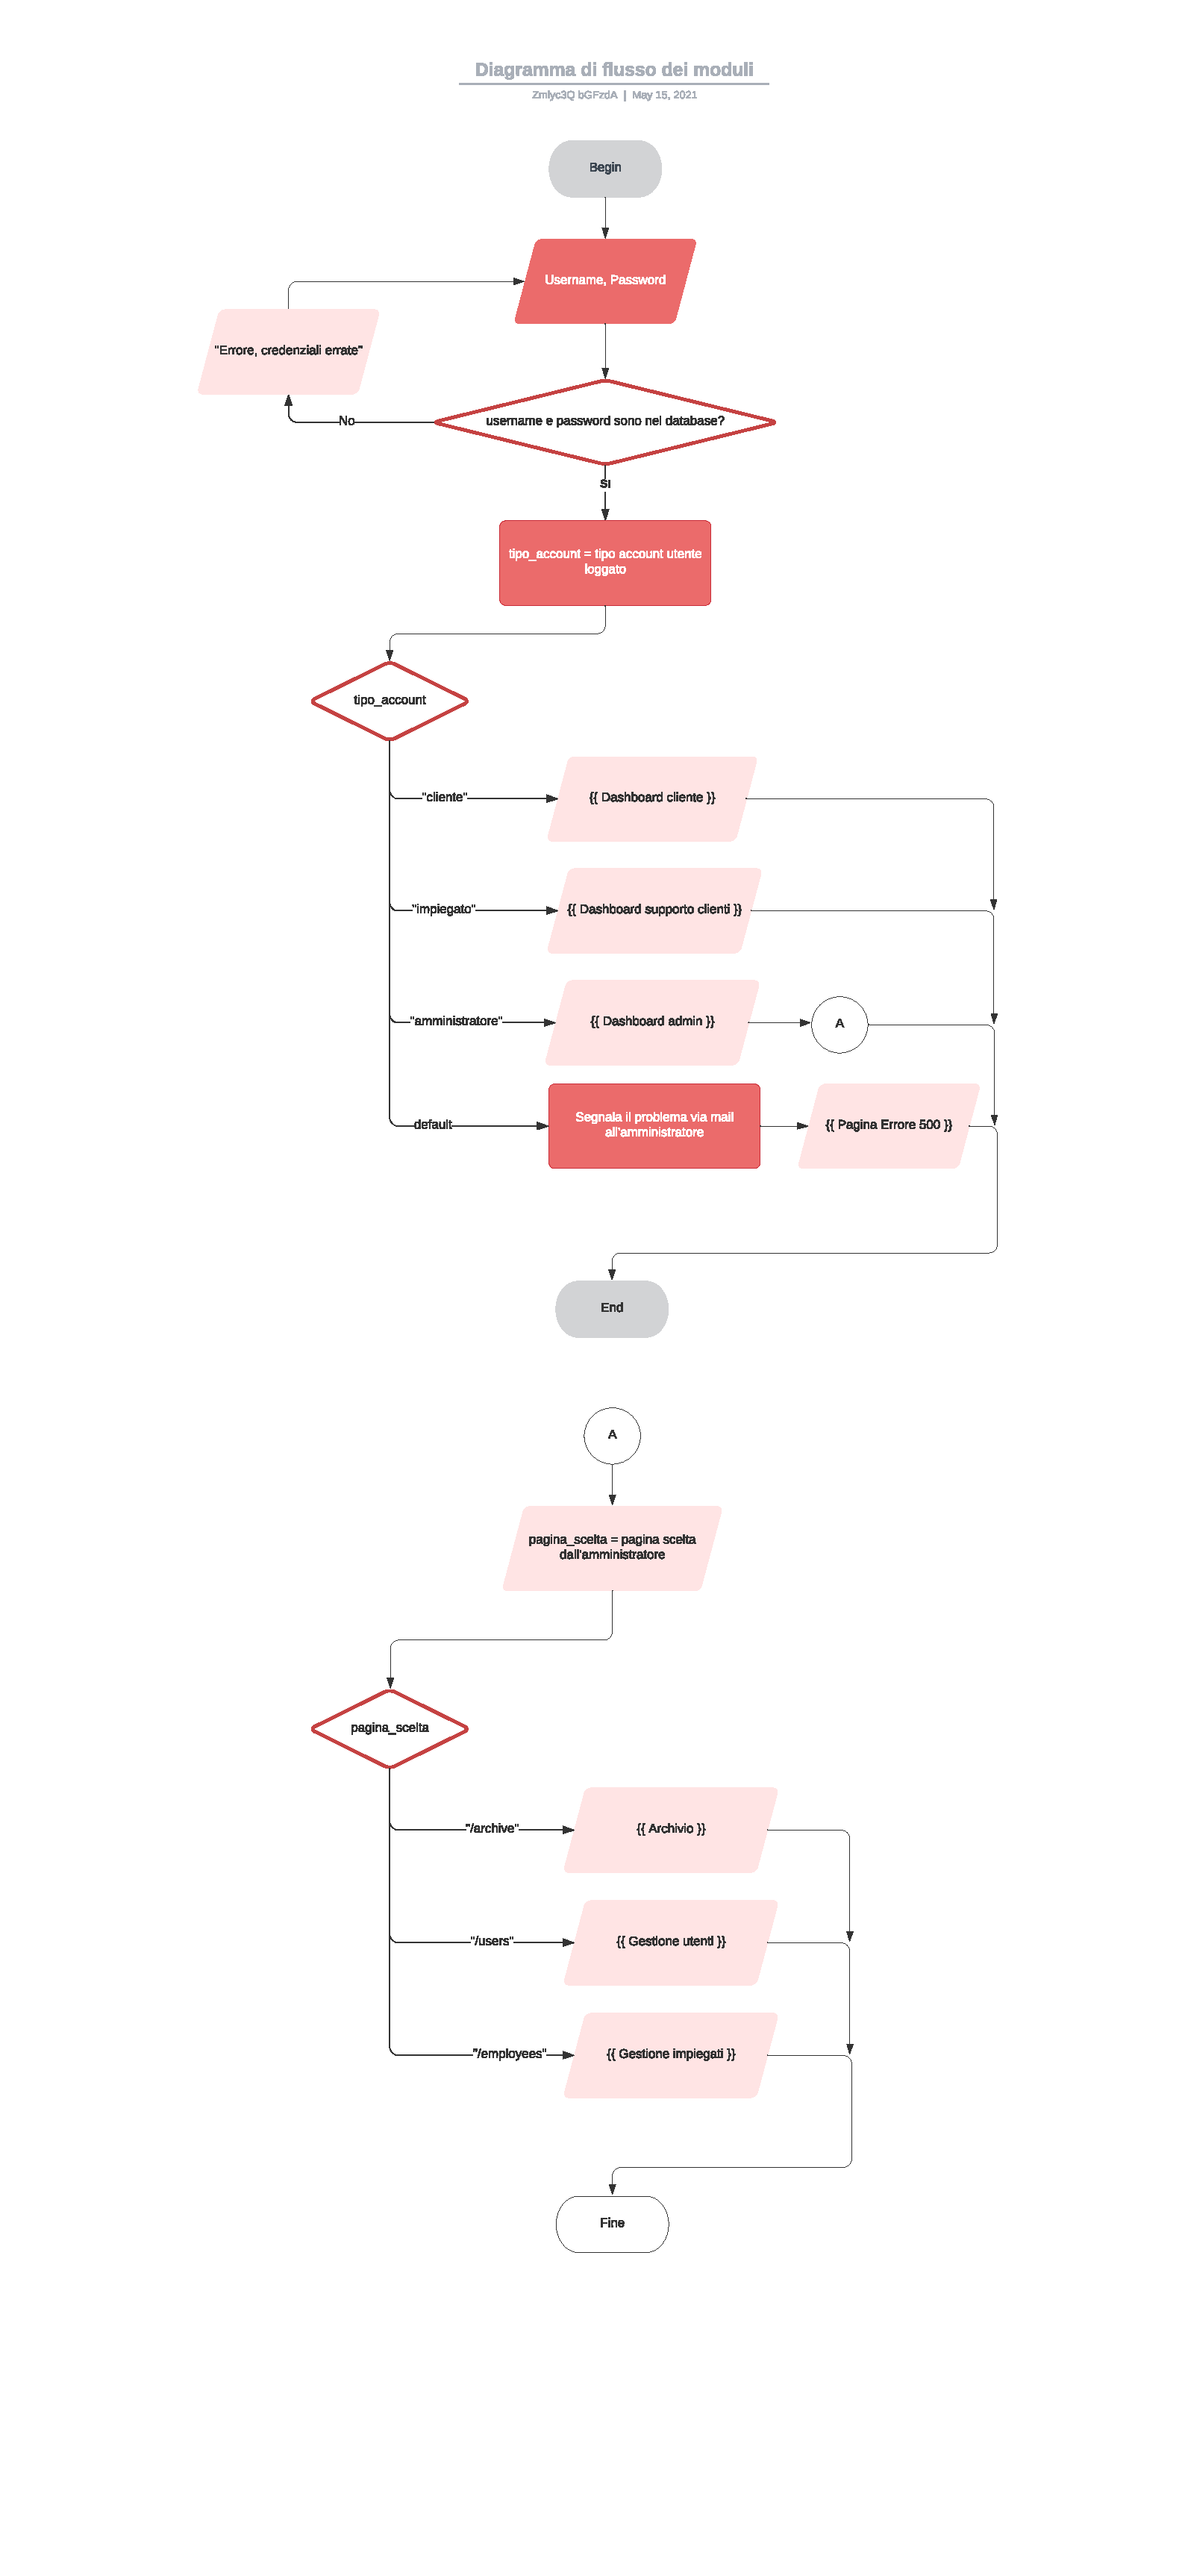
\includepdf{Figures/flow_chart.pdf}